\chapter{Contribuições durante a disciplina}

 Durante a disciplina foram feitas diversas contribuições, que
 culminaram na minha participação no programa Google Summer of Code para colaborar
 com o projeto. Foram enviados e aceitos várias mudanças para
 os repositórios do projeto que contemplam melhorias em documentação, refatorações
 de código, correção de bugs, escrita de testes, e adição de funcionalidades.

 As contribuiçoes foram descritas em um diário e registram as contribuições
 feitas semanalmente ao longo do semestre. O documento (em inglês) está disponível publicamente 
 em um documento do Google Drive no link: \href{https://docs.google.com/document/d/1AsMZK2SeN7W3hJHHK9ZjVmWU83nYqf7LO4NSWKndc7w/edit}{Meu Diário}.

\section{Linha do Tempo}
\label{cap:linha-do-tempo}

 Apresento a seguir uma listagem das contribuições feitas, durante 14 semanas de
 atividades. Os registros iniciam no dia 4 de Março e finalizam em 9 de Junho e
 cada semana vai de domingo até sábado.
 
\begin{figure}
  \caption{\textbf{\underline{Semana 1 (04 de Março - 10 de Março)}}}
  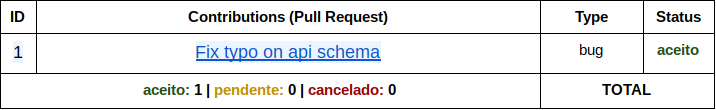
\includegraphics[width=\linewidth]{figuras/contribs-1.png}
\end{figure}

\begin{figure}
  \caption{\textbf{\underline{Semana 2 (11 de Março - 17 de Março)}}}
  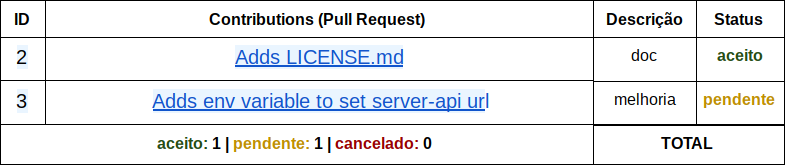
\includegraphics[width=\linewidth]{figuras/contribs-2.png}
\end{figure}

\begin{figure}
  \caption{\textbf{\underline{Semana 3 (18 de Março - 24 de Março)}}}
  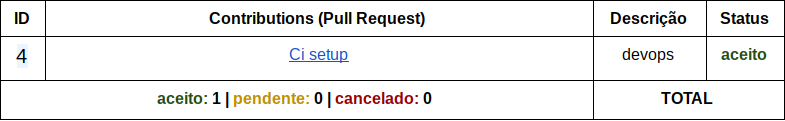
\includegraphics[width=\linewidth]{figuras/contribs-3.png}
\end{figure}

\begin{figure}
  \caption{\textbf{\underline{Semana 4 (25 de Março - 31 de Março)}}}
  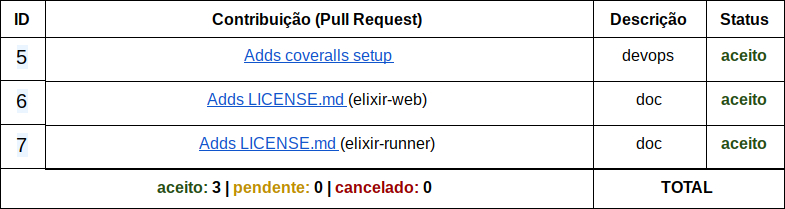
\includegraphics[width=\linewidth]{figuras/contribs-4.png}
\end{figure}

\begin{figure}
  \caption{\textbf{\underline{Semana 5 (1 de Abril - 7 de Abril)}}}
  \centering
  
\includegraphics[width=30mm, scale=0.5]{figuras/loading.png}
\end{figure}

\begin{figure}
  \caption{\textbf{\underline{Semana 6 (8 de Abril - 14 de Abril)}}}
  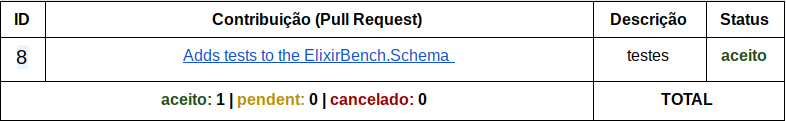
\includegraphics[width=\linewidth]{figuras/contribs-5.png}
\end{figure}

\begin{figure}
  \caption{\textbf{\underline{Semana 7 (15 de Abril - 21 de Abril)}}}
  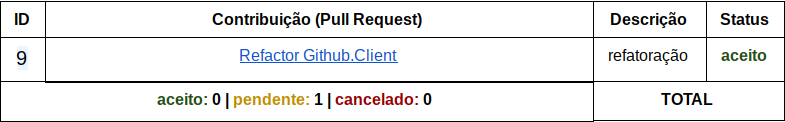
\includegraphics[width=\linewidth]{figuras/contribs-6.png}
\end{figure}

\begin{figure}
  \caption{\textbf{\underline{Semana 8 (22 de Abril - 28 de Abril)}}}
  \caption{\textbf{\underline{Semana 9 (29 de Abril - 5 de Maio)}}}
  \caption{\textbf{\underline{Semana 10 (6 de Maio - 12 de Maio)}}}
  \centering
  
\includegraphics[width=30mm, scale=0.5]{figuras/loading.png}
  \caption{Semanas 8, 9 e 10 trabalhando em contribuições mas sem enviar Pull Requests}
\end{figure}

\begin{figure}
  \caption{\textbf{\underline{Semana 11 (12 de Maio - 19 de Maio)}}}
  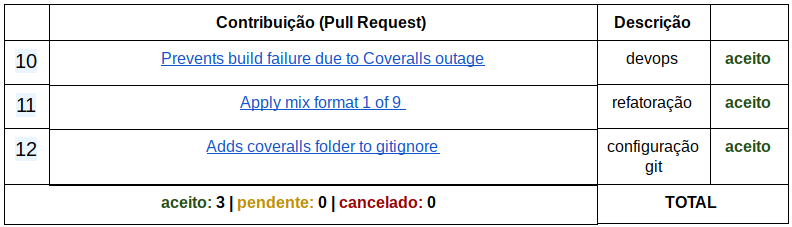
\includegraphics[width=\linewidth]{figuras/contribs-7.png}
\end{figure}

\begin{figure}
  \caption{\textbf{\underline{Semana 12 (20 de Maio - 26 de Maio)}}}
  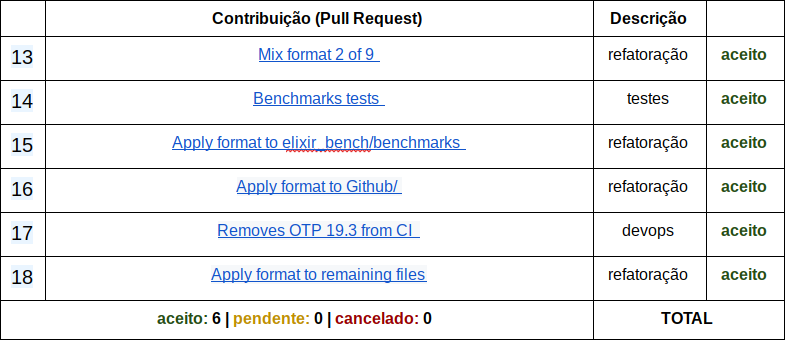
\includegraphics[width=\linewidth]{figuras/contribs-8.png}
\end{figure}

\begin{figure}
  \caption{\textbf{\underline{Semana 13 (27 de Maio - 2 de Junho)}}}
  \centering
  
\includegraphics[width=30mm, scale=0.5]{figuras/loading.png}
\end{figure}

\begin{figure}
  \caption{\textbf{\underline{Semana 14 (3 de Junho - 9 de Junho)}}}
  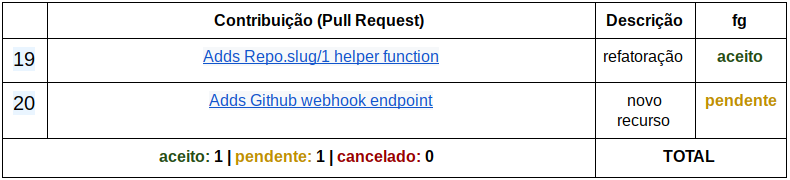
\includegraphics[width=\linewidth]{figuras/contribs-9.png}
\end{figure}

\section{O que aprendi colaborando}
\label{cap:o-que-aprendi}

 Meu aprendizado com o projeto pode ser divido de duas formas,
 um aprendizado técnico e um aprendizado conceitual. Tecnicamente falando,
 aprendi várias tecnologias novas as quais eu não tinha experiência antes, como a
 linguagem de programação Elixir e o paradigma funcional, funcionalidades mais
 avançadas do Docker, biblioteca de API em GraphQL, aplicação frontend desacoplada escrita com o
 framework React, entre outros... o que aumentou bastante meu nível técnico.
 Por outro lado, o domínio do projeto me fez adquirir também um
 certo conhecimento sobre a área de testes e métricas de desempenho, o que me
 levou até a pensar sobre pesquisas científicas na área. Apesar de ser bastante
 conhecimento de uma só vez, foi possível avançar nessa situação tendo como
 exemplo uma aplicação real, através dos códigos já existentes e da interação
 com os própios criadores desses códigos.

 Listar meus conhecimentos adquiridos com o projeto levaria uma grande quantidade
 de palavras. Acredito que hoje sou um desenvolvedor muito melhor por estar
 em contato com esse projeto, em uma nova linguagem, em um novo paradigma de programação
 e em contato com desenvolvedores experientes que discutem ideias e revisam meu trabalho.
